
\chapter{Community effects of fishing}
\label{chap:communityfishing}
\textsc{\refpart{part:populations}} explored the impacts of fishing on demography (\refchap{chap:fishing}), evolution (\refchap{chap:FIE}), and dynamics (Chapters \ref{chap:dynamics} and \ref{chap:consumerresource}).  In this way the theory comprehensively covered all aspects of single fish stock demography needed for developing fisheries advice.  By and large, many of these applications are already serviced by the classic Beverton-Holt age-based theory, with the exception of fisheries-induced evolution and consumer-resource dynamics.  The size-based theory does have some advantages, such as the direct link to physiological traits for data-poor applications and the ability to estimate the recruitment.  Nevertheless, the fisheries applictions developed so far falls short of the promise to deal with species interactions needed for ecocystem-based fisheries management.  We did cover some aspects of species interactions by changing the physiological mortality to represent changes in the wider community leading to altered scope for growth and risk of predation, and by the consumer-resource model in \refchap{chap:consumerresource}.  Such simple considerations may be sufficient in a single-species advice context, however, strategic ecosystem-based management requires a more holistic approach that can directly assess how fishing on one part of the community affects other parts. For example: How does a fishery on cod affect the herring population -- and vice versa?  Or, more generally: how does the development of a forage fishery on small pelagic species affect the yield of a consumer fishery for large demersal species.  Such ecosystem level impact assessments are necessary to quantify the trade-offs between management actions.  Trade-offs between management actions are the cornerstones in strategic management plans of entire ecosystems.

We can divide the effects of fishing into the direct effects on demography and recruitment of the targeted stocks and the indirect effects on other stocks due to the reduction in biomass of the target stocks.  While the direct effects of fishing are fairly straight-forward, assessing the indirect effects involves several processes:  The reduction of the target stock means that competitors will face less competition -- a positive impact on the rest of the fish community.  However, predators on the stock will have to look for food elsewhere -- a negative impact -- while the stocks' prey species will enjoy a safer and more productive life -- a positive impact.  And it becomes even more complex: the release of the prey population from predation will increase their abundance, and they may thereby increasingly compete with juveniles from the target population -- a negative impact on the target stock.  Adding all these effects with different signs to assess the net outcome of the indirect effects of fishing is obviously not straight-forward.   The assessment is further complicated because the indirect effects propagate in all directions in the food-web: individuals at the same trophic level as the target stock face decreased competition, higher trophic levels have less food, and lower trophic levels experience decreased predation.  The community model developed in the previous chapter accounts for all these effects.

Modelling the impact of fishing on an entire community is more complex than the single-stock impact assessments in Chapter~\ref{chap:fishing}.  While considering a single stock in isolation we could make a fairly exhaustive impact assessment by varying the fishing mortality, the fisheries selectivity, and the physiological mortality on all aspects of the stock: biomass, size structure, and recruitment.  A similarly detailed assessment of the entire community is impossible  in this space.  Instead I will focus on three important examples: trophic cascades initiated by the removal of large predators, the trade-offs between a forage fishery and a consumer fishery, and the extension of the Maximum Sustainable Yield (MSY) concept to the community.  Returning finally to the single stock aspects, I will illustrate how the {\Fmsy} on each stock is context-dependent -- it changes with the surrounding community.



\section{Trophic cascades}
\label{sec:cascades}\index{Trophic cascade|(}
When a component of an ecosystem is perturbed the effects are not isolated to the component itself but cascades through the ecosystem, much like the waves from a rock thrown into a pond propagate away from the point of impact.  Perturbations are mainly propagated through the predator-prey interactions: if a predator is removed it releases the prey from predation, leading to an increase in the prey population, which then induces a higher predation pressure on the preys prey etc..  Such trophic cascades are the signature of indirect effects of changes in the abundance of individuals in one trophic level on other trophic levels. The previous chapter gave us an example where the high abundance of large fish led to a higher predation pressure on their prey  (\reffig{fig:DynamicCommunity}).  

% Trophic cascades are indeed observed in fish communities: in the Black Sea \citep{Daskalov2007}, the Baltic Sea \citep{Casini2008, Mollmann2008}, and the Northwest Atlantic \citep{Frank2005, Myers2007}.  In these cascades the removal of large fish led to increases in forage fish, which in turn caused decreases in zooplankton.  

\begin{figure}[t]
  \centering
  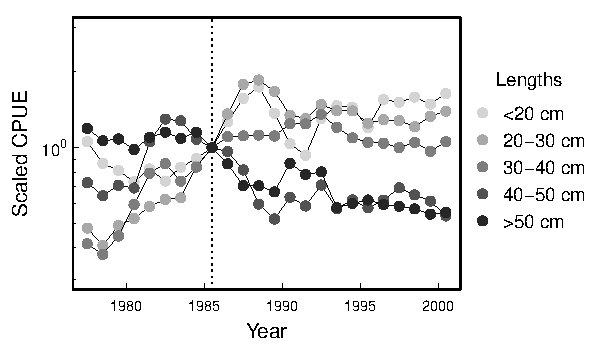
\includegraphics{ChapterCommunityFishing/Daan.pdf}
  \caption{Catch-per-unit-effort (CPUE) from international bottom trawl survey in the North Sea organised according to length groups.  All data-points are normalized with the value in 1985.  Data from \citet{Daan2005}.}
  \label{fig:Daan}
\end{figure}

A classic example of a trophic cascade is the predation by sea otters on sea urchins in the Aleutian archipelago \citep{Estes1998}.  The sea otters appetite for sea urchins kept the urchin population low, such that they were unable to graze down the kelp forest.  This balance was maintained until killer whales developed a taste for sea otters.  The killer whales then decimated the population of sea otters by a factor of 10 in less than a decade.  The result was a huge bloom in sea urchins whose increased grazing pressure led to the disappearance of kelp forests.  In this example the trophic cascade spanned four trophic levels with a strong effect all the way down to the primary producers.  Similar cascades have been observed among fish communities.  On the Scotian Shelf Ken \citet{Frank2005} reported the effects of disappearing groundfish stocks (largely cod) over a 20 year period.  Prey species of shrimp, snow crabs, and forage fish responded to the relaxed predation pressure by increasing abundances, most pronounced among the forage fish.  Increased populations of forage fish led to decreases in large zooplankton, which again resulted in higher concentrations of phytoplankton.  A similar cascade was observed in the Baltic Sea where there collapse of the cod stock lead to increases in sprat populations and decreases in zooplankton \citep{Casini2008}.  The observation of trophic cascades is a reminder that a perturbation on one part of the fish community -- for example the largest fish -- has ecosystem-wide repercussions. 

The trophic cascades can also be observed as changes in the size distribution of the community.  By analysing trawl survey data from the North Sea, \citet{Daan2005} saw that small-bodied fish increased in abundance while large-bodied fish decreased over a 20 year period (\reffig{fig:Daan}).   These changes -- decrease in large fish leading to a decrease in small fish -- have often been described as changes in the size spectrum exponent \citep{Rice1996, Bianchi2000, Daan2005}, or the ``large fish indicator'', which is the ratio of biomass of individuals smaller and larger than 40 cm \citep{Greenstreet2010, Blanchard2014}.  Both of these indicators can be deceptive, however, as they cannot distinguish between a trophic cascade that leads to an increased numbers of small fish and one that is just a reduction in the abundance of large fish (see Fig.~6 in \citet{Andersen2010} for an illustration of this effect). 

\afterpage{\clearpage}
\begin{figure}[p]
  \centering
  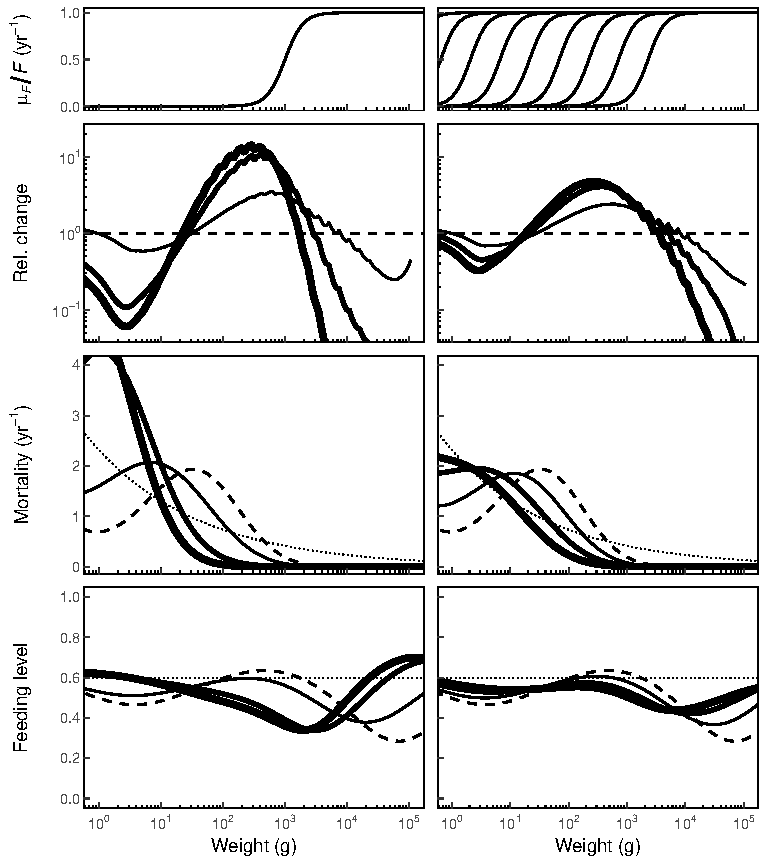
\includegraphics{ChapterCommunityFishing/Cascades.pdf}
  \caption{The impact of fishing the un-exploited community from \reffig{fig:DynamicCommunity} (dashed lines) with two types of fishing (top row): fishing only individuals larger then around 1 kg (left column), or fishing all species with a trawl selectivity starting around 0.05 of asymptotic size (right column).  The fishing mortality is $F=0.1$, 0.3 and 0.7 yr\per, shown with increasing line width.  Dotted lines represent theoretical expectations and the dashed lines are the unexploited situation.  The second row show the community size spectrum relative to the unfished spectrum, $N_c(w)/N_c(w, F=0)$.}
  \label{fig:Cascades}
\end{figure}
 
To explore how the modelled community responds to fishing, I expose it to two patterns of fishing in \reffig{fig:Cascades}: fishing only on large individuals irrespective of species (left column) and fishing on all species with a trawl-like selectivity pattern (right column).  The first pattern corresponds roughly to the situation on the Scotian shelf where the fishery is concentrated on the large demersal species, while the second pattern resembles the exploitation in a fully developed fishery where all species are full exploited, like the North Sea.  In both cases the model responds with a trophic cascade of the sort seen in the data discussed above: larger individuals decline, which leads to an increase in smaller fish and possibly, only in the first case, to a reduction in the zooplankton community.  

The trophic cascades are first and foremost driven by changes in predation pressure: the mortality in the range 10 to 1000 g becomes smaller while the mortality on sizes less than 10 g is increased (third row).  The growth rate also has a role to play.  Notice how the abundance of fish around 1000 g is increased relative to the unfished case despite being fished.  The increase happens because of the higher amount of biomass entering the fished range due to the increased abundance of individuals in the size range below 1000 g.  In this way, growth of individuals acts as a dampening mechanism on the trophic cascade.  Therefore the trophic cascade is damped as it moves down the trophic levels \citep{Andersen2010}.  Finally, changes in growth rate plays a role, but it is somewhat minor because the changes are fairly small (last row of panels).  An increase in abundance in a range leads to higher food competition, lower abundances of prey and decreasing feeding levels and slower growth rates.  In a size range where growth slows down, i.e., where $\dd f/\dd w < 0$, biomass piles up because it leaves a size range at a slower rate than it enters a size range.  In the first fishing pattern, this occurs in the size range from about 1 to 500 g, and it therefore increases the abundance in that size range.  The effect is, however, not sufficiently strong to counteract the dampening effect of the cascade by the growth between trophic levels. \index{Trophic cascade|)}





\section{What is the impact of forage fishing?}%Interaction between fisheries}
\index{Fishing!Forage|(}
The analysis of data and model simulations speaks clearly: the removal of large fish by fishing has released small fish from predation pressure.  The resulting increase in forage fish biomass has facilitated the expansion of forage fisheries.  The question is, then, whether the interaction goes both ways.  Will a developed forage fishery limit the productivity of large fish species \citep{Houle2013, Ravn-Jonsen2016}?  If that is the case, the developed forage fisheries will reduce the economic potential of the valuable demersal stocks or even hinder the recovery of those stocks.

\begin{figure}[t]
  \centering
  \includegraphics{ChapterCommunityFishing/ForageFishing.pdf}
  \caption{Yield from fishing as a function of the forage fishery ($5$ g $\le \W < 150$ g) and the consumer fishery ($\W \ge 150$ g).  Yield is from a) the forage fishery, b) small pelagic fish ($150\, \mathrm{g}\, \le \W < 5$ kg), and b) from large demersal fish ($\W \ge 5$ kg). The white area is where one species in each group has been fished to extinction.}
  \label{fig:foragefishing}
\end{figure}

To examine the interaction between forage and consumer fisheries I have defined three fisheries: a forage fishery targeting small species ($5$ g $\le \W < 150$ g \footnote{I have omitted the smallest species $\W=4$ g from being eposed to forage fishing. Those small species are very vulnerable to fishing and quickly goes extinct.}), a pelagic fishery target targeting medium sized fish ($150\, \mathrm{g}\, \le \W < 5$ kg), and a consumer fishery targeting large fish ($\W \ge 5$ kg).  I calculate the yield from each fleet as a function of the fishing mortality on the forage fishery and on the two fisheries targeting fish for consumption (the pelagic and demersal fisheries; $\W > 150$ g) (\reffig{fig:foragefishing}).  

The yield from the forage fishery (the first panel) increases as the fishing pressure in the consumer fishery is increased.  This, again, illustrates how the consumer fishery facilitates the forage fishery.  Turning to the yield from the fishery on large fish (last panel), we see that the contour lines are almost parallel to the x-axis, signifying that the yield is largely independent of the fishing pressure on the forage fish.  Only if the fishing mortality in the consumer fishery is very high -- around 1 yr{\per} -- does the model show a small negative effect of a heavy forage fishery.  In other words: the forage fishery does not have a strong impact on the consumer fishery. 

The limited dependence of the large fish on forage fish runs counter to our intuitive mental picture of a simple food-chain: removing a basal resource -- here the forage fish -- is expected to pull the carpet away from under all higher trophic levels.  However, the fish community cannot be perceived as a simple food-chain: even fish with a large asymptotic size start their life as tiny larvae.  Therefore the removal of fish with small asymptotic size (the forage fish) releases the juvenile individuals from species with larger asymptotic size from competition.  In this way, adults of the large species are compensated by the lack of forage fish prey by higher juvenile growth rates and by higher abundance of juvenile and adult medium sized fish\note{Consider a figure showing spectra for two cases: one with zero forage fishery and one with high forage fishery}.  To which degree does this result reflect the reality of competition of predator-prey interactions in a natural ecosystem?  For instance, does juvenile from large-bodies fish species share a habitat and compete for food resources with adult forage fish?  Probably not to the degree assumed in model.  Nevertheless, we can conclude that the propagation of trophic cascades depends upon the direction: perturbations on a high trophic level cascades down the trophic levels with a small damping for each step.  Perturbations on lower trophic level species has a limited effect upon higher trophic level species.
\index{Fishing!Forage|)}


\section{What is the maximum sustainable yield of a community?}
\label{sec:communityMSY}
Maximizing the yield seems like a straight-forward exercise: calculate the yield as a function of fishing mortality and find the maximum -- just as we did for the single stock in \reffig{fig:fishingcomplete}.  Things are more complicated when the entire community is considered: we need to specify how fishing mortality is distributed between species in the system.  

\begin{figure}[t]
  \centering
  \includegraphics{ChapterCommunityFishing/yield.pdf}
  \caption{Yield and biomass of a community where all species are fished with the same fishing mortality.  (a) Total yield (black), total biomass (grey), fraction of species collapsed ($F < \Flim$, see page \pageref{lab:Flim}; thin dashed), and fraction of species with $R_0 < 1$ (thick dashed).  (b) Spawning stock biomass as a function of asymptotic size relative to the biomass in the unfished situation.  The thick contour line show where biomass is equal to unfished biomass; white/black contour lines show higher/lower biomasses by a factor 2 and 5.}
  \label{fig:YieldvsF}
\end{figure}

Before going into that complication we can explore the yield from the system when all species are fished with the same fishing mortality (\reffig{fig:YieldvsF}a).  The total yield (solid line) and the biomass has a similar pattern than in the single species case (\reffig{fig:fishingcomplete}): yield is parabolic with a well-defined maximum, and the total biomass declines (grey line).  The maximum is, however, at a much higher fishing mortality than we found in \refchap{chap:fishing} -- around 2 yr{\per} in contrast to around 0.3 yr{\per} when a single population is exploited (\reffig{fig:refpoints}a).  How can it be that the total community apparently can be exploited much harder than a single species?  The answer lies in the redistribution of predation mortality in the community, just like the trophic cascades (\reffig{fig:YieldvsF}b): the large-bodied species are most vulnerable to fishing, and are over-exploited at fairly low fishing mortalities (just like we saw in the single-species calculations in \reffig{fig:refpoints}a).  This releases the intermediate-sized species from predation pressure so that they, despite being fished, increase in biomass by up to a factor 5. This is the same effect we saw from the trophic cascade in \reffig{fig:Cascades}.  The smallest species, which are also fairly vulnerable to fishing mortality (\reffig{fig:refpoints}a), are met with the double whammy of increased competition from the intermediate-sized species combined with high fishing mortality, and consequently they decline in biomass.  Eventually, at fishing mortality larger than about 0.5 yr\per, the community consists almost exclusively of intermediate-sized species.  Even though the diversity of the community is impoverished, the yield from the fishery is high because there are no losses of these highly productive species to predation by larger species.  The situation may seem academic -- why would we want to over-exploit the system to that degree?  It has, however, been realised in practise in the East China Sea resulting in a fishery with a surprisingly high yield \citep{Szuwalski2017}. The situation is reminiscent of the way agriculture is organized: by removing grazers from crops and predators from herbivores, the production is only determined by the productivity of the basal resources (nutrients, water and climate), and not by losses to higher trophic levels.

\begin{figure}[t]
  \centering
  \includegraphics{ChapterCommunityFishing/communityMSY.pdf}
  \caption{The maximum sustainable yield achieved from the community as a function of the average fishing mortality (black line).  The distribution of effort between three fleets targeting small, medium or large species are indicated with thin, medium and thick grey lines. }
%The division of effort between the three fleets is done by optimizing total biomass yield (left) and optimizing biomass yield under the constraint that the biomass is not allowed to fall below 20\% of unexploited biomass for any species (b).
%Note the logarithmic x-axis that differs from \reffig{fig:yield} to emphasize the fishing pattern at low exploitation rates.}
  \label{fig:communityMSY}
\end{figure}

\index{Maximum Sustainable Yield!Community}How should fishing effort be distributed between species in a community in order to achieve the highest biomass yield from the fishery?  This question confronts an omnipotent manager of all fishing fleets in an ecosystem (\reffig{fig:communityMSY}).  The yield increases with fishing mortality, just as when all species are evenly exploited in \reffig{fig:YieldvsF}.  At high fishing mortality, the division of effort between the three fleets is fairly even.  At small fishing mortalities, however, the pattern of exploitation is different.  Fishing initially targets the large-bodied species. Only when the biomass of these species is reduced, is it favourable to develop a forage fishery.  The largest species are initially targeted because they have the highest biomass.  When the biomass of the largest species is reduced, the situation resembles the trophic cascade in \reffig{fig:Cascades}a: the depletion of large individuals releases smaller individuals from predation pressure.  This increase in smaller species then facilitates the development of a forage fishery.  Eventually, all species are exploited with approximately similar exploitation rates. 

Ecosystem based fisheries management is about much more than maximizing the yield from the fishery.  It is also about conservation of diversity, about securing a high economic rent of the exploitation, and about ensuring a fair distribution of the benefits throughout society.  Some of these aspects can be addressed with the trait-based modelling approach.  We can, for example, clearly see that striving to obtain the community maximum sustainable yield would be incompatible with the aims of ecosystem based management because it entails that many species groups are over-exploited and that the remaining community is impoverished relative to the unexploited community.  Economic aspects can be addressed by modelling rent as the difference between the revenue and the costs of fishing \citep{Gordon1954, Schaefer1954, Clark1973}.  The revenue should account for larger fish typically taking a higher price per kilo than smaller ones \citep{Andersen2015} --  a kilo of bluefin tuna is much more valuable than a kilo of sprat.  Evidently, an ecological model cannot in itself address issues of equal and fair distribution of resources in society, however, models can be used to provide the ecological baseline that are needed for socio-economic considerations and models.  


\begin{figure}[t]
  \centering
  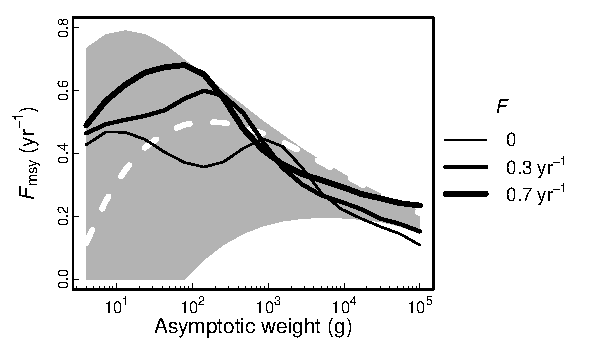
\includegraphics{ChapterCommunityFishing/RefvsF.pdf}
  \caption{The fishing mortality leading to the maximum sustainable yield ({\Fmsy}; see \refsec{sec:refpoints}), as a function of asymptotic size. The lines show three levels of fishing on the community: $F = 0$, $0.5$ and $1.0$ yr\per, corresponding to the communities in \reffig{fig:YieldvsF}. The white dashed line show the prediction from the single-species model from \reffig{fig:refpoints}, and the grey patch is the range of {\Fmsy} if the physiological mortality constant is varied by $\pm 0.15$ (see \reffig{fig:refpointsvsa}).}
  \label{fig:RefvsF}
\end{figure}

Finally, we can explore how fisheries reference points are affected by the changes in the community induced by fishing (\reffig{fig:RefvsF}).\index{Reference points}  We already did this in a crude way in \refchap{chap:fishing} when we represented changes in the community by varying the physiological mortality (\reffig{fig:refpointsvsa}).  The fishing mortality leading to the maximum sustainable yield {\Fmsy} for each species roughly follows the same pattern as the single species calculations (\reffig{fig:refpoints}).  In general the reference points increase as the community is fished harder.  The higher productivity is facilitated by release of predation by larger species and diminished competition, both results of the lower biomass in the community.  We can also see that the changes in {\Fmsy} are not entirely systematic; some species groups are even predicted to tolerate lower fishing mortalities ({\W} around 1 kg).  It is therefore difficult to formulate general rules, however, the results once again highlight that fisheres reference points and the productivity of fish stocks are not constant properties of the fish stocks themselves. Fisheries reference points are context dependent -- they change in tune with the dynamics of the surrounding fish community.  Enlightened fisheries management therefore need to revisit calculations of references point continually.



\section{Size- and trait-based models for ecosystem-based fisheries management}
I have shown how the trait-based size spectrum model can be used to explore the effects of fishing on the entire ecosystem.  Charles \citet{Elton1926} wrote in his classic Animal Ecology: \emph{``The food-relations of animals are extremely complicated [ \ldots ] it is usually quite impossible to predict the precise effects of twitching one thread in the fabric''}.  He was right, and we are still unable to accurately predict the dynamics of a specific species in a food-web.  However, by lumping species with similar traits -- in this case similar asymptotic sizes -- the trait-based size spectrum model generates robust predictions of how the size- and trait-structure is affected by perturbations.  This makes the model suitable as a tool for ecosystem based fisheries management.

The ``Ecosystem Approach to Fisheries Management''\index{Ecosystem approach|(}  was born out of a realisation that the current approach of single-stock fisheries management is inadequate to deal with interactions between fish stock \citep{May1979}.  The ecosystem approach has been formalised in international agreements \citep{FAO2003} and has been adopted to various degrees and in different ways around the world.  The European Union has developed the Marine Strategy Framework Directive with the goal of ``clean, healthy, and productive oceans'' by 2020, the US has tried a variety of approaches \citep{Essington2016}, and Australia has been noted for its implementation ecosystem approaches to fisheries management, which has improved the sustainability of fished stocks \citep{Smith2007b}.  The ecosystem approach takes a holistic view of fisheries management by considering the entire ecosystem and not only the fish.  The approach accounts for all uses and constraints of the ecosystem: production of food, generation of economic value, conservation of ecosystem function, habitats, and biodiversity, as well as equal division of ecosystem benefits among users.  The goals are ambitious, and predictably management has struggled to achieve them.  For one, the institutional challenges are enormous.  Followed to the letter, the ecosystem approach mandates that all stakeholders -- fishers, consumers, NGOs, scientists, politicians etc. -- are engaged in the process.  Getting them to agree at the same table is not straight-forward.  The other problems are practical: we need adequate tools to make impact assessments of management actions on the ecosystem level.

Which tools does the ecosystem approach need?  It is tempting to call for a replacement of single-stock models in advice with a ecosystem-oriented advice based on food-web models.  However, it is clear that  single-stock management will not -- and should not -- go away.  We still need specialised working groups who know the intricacies of each specific stock, and we still need them to make single-stock stock assessments, impact assessments, and management plans.  What the ecosystem approach needs is to embed these plans within a consideration of the entire ecosystem and develop ``fisheries ecosystem plans''\index{Fisheries ecosystem plans}, as described by the Lenfest fishery ecosystem task force \citep{Essington2016}.   Ecosystem management plans should constrain the actions of single-stock management to avoid single-stock actions that is beneficial for a specific stock, but creates unacceptable outcomes for other components of the ecosystem.  A good example is reverse trophic cascades:  when formerly overfished fish stocks recover they impose an increasing predation pressure on forage fish.  As a result, the productivity of forage fish stocks is reduced to the detriment of forage fisheries and other dependent predators such as a birds and mammals \citep{vanGemert2018}.  Avoiding, or preparing, for such eventualities requires that the strategic objectives of fisheries management at the ecosystem level are explicitly formulated.  

A focal point in a fisheries ecosystem plan a vision of the ecosystem we want.  From a fisheries perspective the immediate answer might be: one which provides the maximum sustainable yield (MSY).  However, MSY for the fishing fleets might compromise the needs of other dependent species, such as birds or marine mammals.  Further, as we saw in this chapter, MSY in a community context is not straightforward -- it is certainly different than just MSY for all the single stocks because the MSY of a stock is highly sensitive to the changes in predation pressure and, to a smaller extent, food availability \citep{Rindorf2016}.  The key is that there are trade-offs between management actions, and that struggling to achieve one goal may compromise others \citep{Link2010}.  Ecosystem models offer an appealing tool to explore some of the trade-offs between ecosystem management objectives to help develop a realistic vision for the ecosystem.

A central concern about model choice for fisheries ecosystem plans is the balance between complexity and simplicity.  A complex modelling approach attempts to represent all processess in and around the ecosystem, from physics to socio-economics, at as fine scale as possible, temporal, spatially, and as many species as possible.  An impressive example of this approach is the development of the ecosystem model system Atlantis\index{Atlantis} \citep{Fulton2011}, which have been set up for ecosystems around the world.  Such models provide stakeholders all the information they want and makes it possible to generate scenarios of management actions to explore the trade-offs -- the costs and benefits -- of management actions on the entire system.  They are, however, also monstrous beasts to set up and operate.  Calibration of such models for a given system requires several man years and running scenarios takes hours or days.  What is more troublesome is their complexity.  Due to the large number of parameters and processes, many of which are poorly known, one is never sure whether all important processes are adequately resolved or whether there is a devil hidden in some detail.  Their outputs of beautiful maps are beguiling to the viewer, but the interpretation of the robustness of results is difficult.  Despite these problems, a well-calibrated model does generate useful output.   Further, the level of detail makes them very well suited as tools to communicate with stake-holders.  At the other end of the complexity-simplicity spectrum are very simple food-web motif models, such as predator-prey models or trophic chains.  These models can be used for generic impact assessments (see e.g.~\citet{Matsuda2006}).  The advantages of such models are their very simple formulation with each process being clearly visible, and they are fast and easy to simulate and analyse.  On the down-side the models are poor representations of real ecosystems and they are difficult to parameterise to provide reliable quantitative estimates of rates and quantities like reference points.  While such model have a place in the primary scientific literature, they are rarely used for operational fisheries management.  

The size-spectrum model I have developed here is sandwiched between the complex end-to-end ecosystem models and the conceptual food-web models.  The size-spectrum model only represents one aspect of the ecosystem -- the fish community -- and it does not resolve specific species but represent diversity through variation in the governing trait.  However, the model is carefully derived from the individual-level processes described in Chapters \ref{chap:sizespectrumtheory} and \ref{chap:individual} and can produce credible quantitative estimates.  In this chapter I developed two examples of trade-offs between management actions: the initiation of a trophic cascade when large fish are over-exploited, and the conflict between fisheries between forage fish and large fish.  The exploration indicated some less obvious effects, in particular that a moderate forage fishery only has a limited effect on the large species.  Other explorations of ecosystem effects of fishing with the model are species recovery \citep{Andersen2010b}, pareto efficiency \citep{Jacobsen2017}, and evaluation of ``balanced harvesting'' \citep{Jacobsen2014, Kolding2016}

A good example of an attempt to make a generic fisheries ecosystem plan is the concept of ``balanced harvesting'' \citep{Zhou2010}\index{Balanced harvesting}.  The idea of balanced harvesting is to distribute fishing mortality across all ecosystem components in proportion to their natural productivity in order to preserve size and species composition of the ecosystem \citep{Garcia2012}.  This definition is unclear on three aspects.  First, it mixes an objective -- preservation of ecosystem composition -- with the method -- fishing proportional to productivity.  Second, it is unclear what is meant by ``productivity''.  A productivity is generally defined as the production of a system relative to the unit of production. In fisheries the unit of production is the fish stock, so the productivity is the production (the yield) per biomass (spawning stock biomass or fished biomass), with dimensions of time\textsuperscript{-1}.  As we have seen repeatedly, measures related to the productivity, be it the population growth rate $\rmax$ or the fishing mortality at maximum sustainable yield, are highly context sensitive.  A productivity is therefore not a biological property of a given stock or species, but it depends on the ecological context, in particular the amount predators.  Further, there has been confusion as how to define the unit of production, with some maintaining that the unit of production is an area, such that the productivity is the production per area with dimensions mass per time \citep{Law2012, Law2013}.  While it is a valid interpretation of the word ``productivity'', it is a clearly a very different measure than the production per unit biomass.  Third, it is not entirely evident how to define the productivity of a size class.  This lack of precision in the definition has led to confusion about what exactly constitues balanced harvesting: is it a strategy which preserves ecosystem structure, or is the act of fishing proportional to productivity (whatever the definition).  Clearly, balanced harvesting in its current form does not constitute a strategic plan that can be operationalised as a fisheries ecosystem plan.  It is, however, the first such formulation of general principles for a plan, and as such it makes a starting line for formulating strategic fisheries ecosystem plans.

The size-spectrum model framework is not the one tool to fill all the needs of ecosystem-based fisheries management.  What it can do is make simple strategic ecosystem oriented assessments of management trade-offs, which are needed to make strategic fisheres ecosystem plans.  It can also with a modest effort be calibrated more closely to resolve specific species in a given ecosystem \refbox{box:foodwebmodel}, and be used for specific ecosystems \citep{Jacobsen2017}.   Simulations with the model highlight how everything in the community is connected and the dynamic nature of the fisheries reference points.  Fisheries management tends to treat the fisheries reference points and the productivity of stocks as fixed properties of the species.  A concrete task for ecosystem based fisheries management is to provide the single-stock advice process with information about how changes in the fish community affects the mortality, and thereby the reference points, for all stocks.\index{Ecosystem approach|)}
